\documentclass{beamer}

\usefonttheme{professionalfonts} % using non standard fonts for beamer
\usefonttheme{serif} % default family is serif

\usepackage{hyperref}

%\usepackage{minted}

\usepackage{animate}

\usepackage{graphicx}

\def\Put(#1,#2)#3{\leavevmode\makebox(0,0){\put(#1,#2){#3}}}

\usepackage{color}

\usepackage{tikz}

\usepackage{amssymb}

\usepackage{enumerate}


\newcommand\blfootnote[1]{%

  \begingroup

  \renewcommand\thefootnote{}\footnote{#1}%

  \addtocounter{footnote}{-1}%

  \endgroup

}

\makeatletter

%%%%%%%%%%%%%%%%%%%%%%%%%%%%%% Textclass specific LaTeX commands.

 % this default might be overridden by plain title style

 \newcommand\makebeamertitle{\frame{\maketitle}}%

 % (ERT) argument for the TOC

 \AtBeginDocument{%

   \let\origtableofcontents=\tableofcontents

   \def\tableofcontents{\@ifnextchar[{\origtableofcontents}{\gobbletableofcontents}}

   \def\gobbletableofcontents#1{\origtableofcontents}

 }

%%%%%%%%%%%%%%%%%%%%%%%%%%%%%% User specified LaTeX commands.

\usetheme{Malmoe}

% or ...

\useoutertheme{infolines}

\addtobeamertemplate{headline}{}{\vskip2pt}



\setbeamercovered{transparent}

% or whatever (possibly just delete it)

\makeatother

\begin{document}
\title[DCEL report]{RIDIR Report}
\author[AC]{Andres Calderon}
\institute[Fall'19]{University of California, Riverside}
\makebeamertitle
\newif\iflattersubsect

\AtBeginSection[] {
    \begin{frame}<beamer>
    \frametitle{Outline} 
    \tableofcontents[currentsection]  
    \end{frame}
    \lattersubsectfalse
}

\AtBeginSubsection[] {
    \begin{frame}<beamer>
    \frametitle{Outline} 
    \tableofcontents[currentsubsection]  
    \end{frame}
}

\begin{frame}{Working on Edge Partitioner}
{Modifiying DCEL local construction}
    \begin{enumerate}
        \item Extract edges from polygons after they are read.
        \item Partition Edge records:

        {\footnotesize \texttt{Edge \{line: LineString, id: Int, ring: Int, order: Int\} } }

        \item Extract edges from the cell.
        \item Merge cell and polygon edges.  Find intersections.
        \item Build the DCEL at local level\footnote{Work in progress}.
    \end{enumerate}
\end{frame}

\begin{frame}{Demo test}
    \centering 
    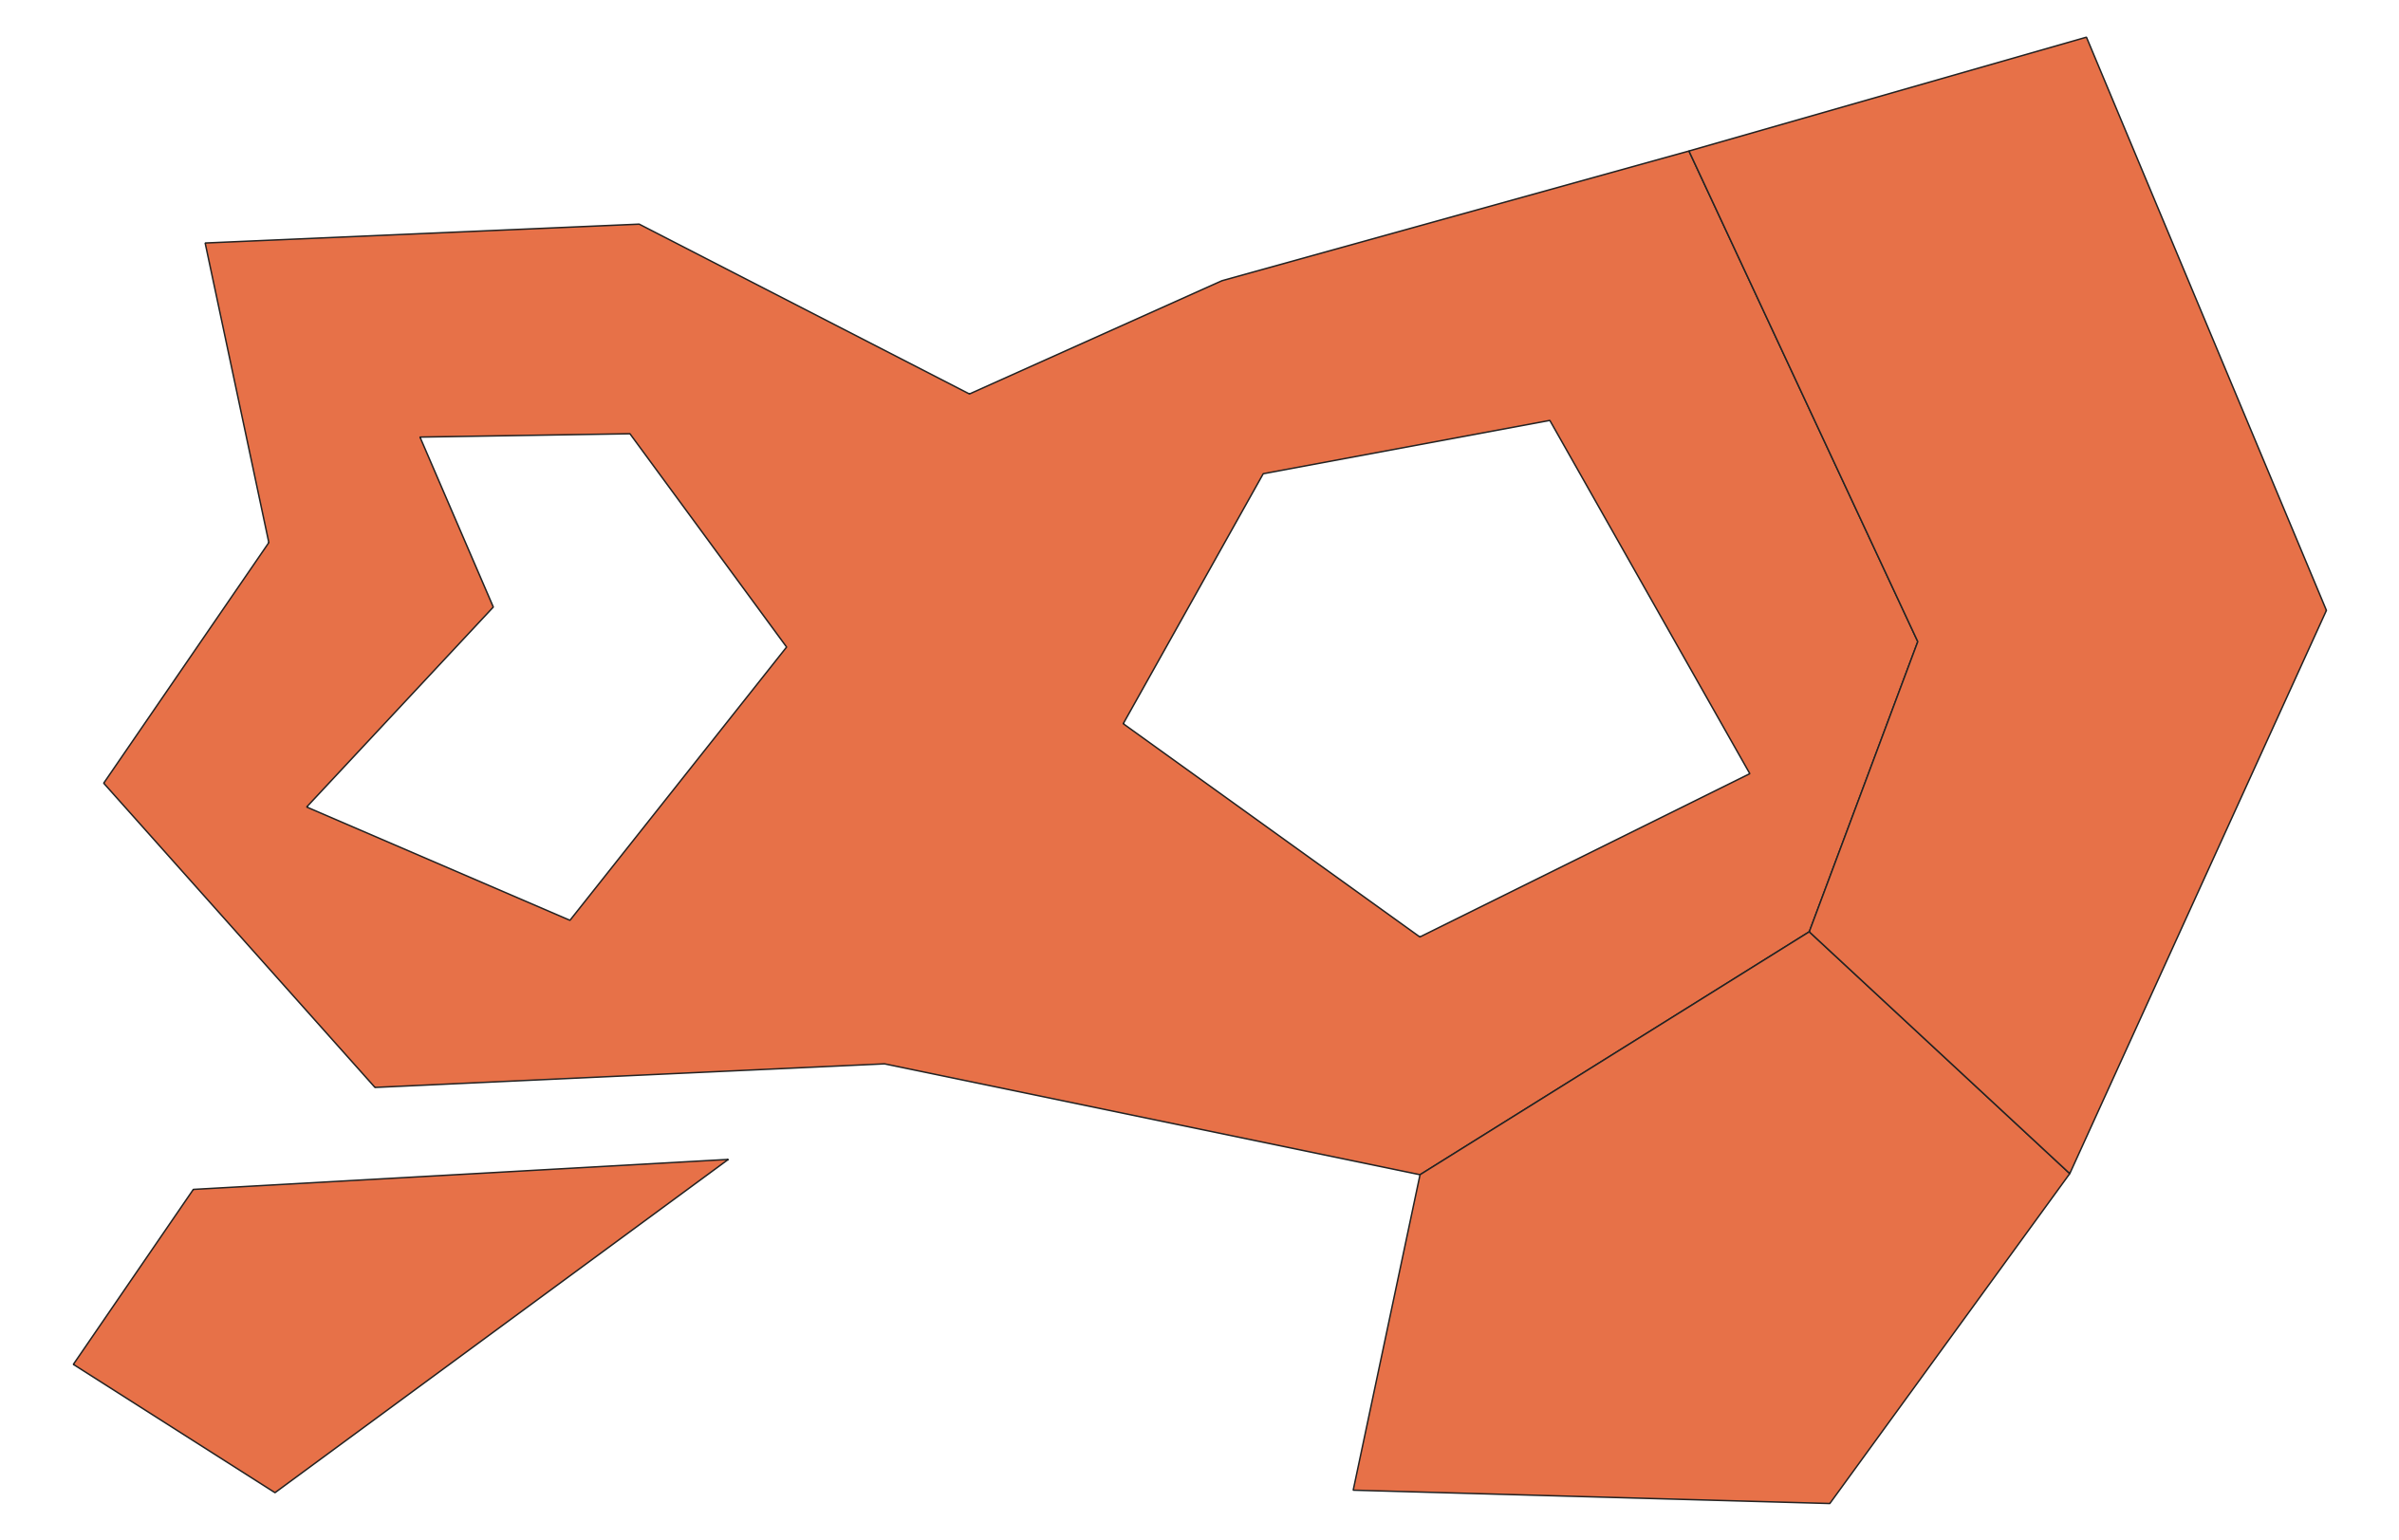
\includegraphics[width=0.8\linewidth]{figures/EP01}     
\end{frame}

\begin{frame}{Extract edges}
    \centering 
    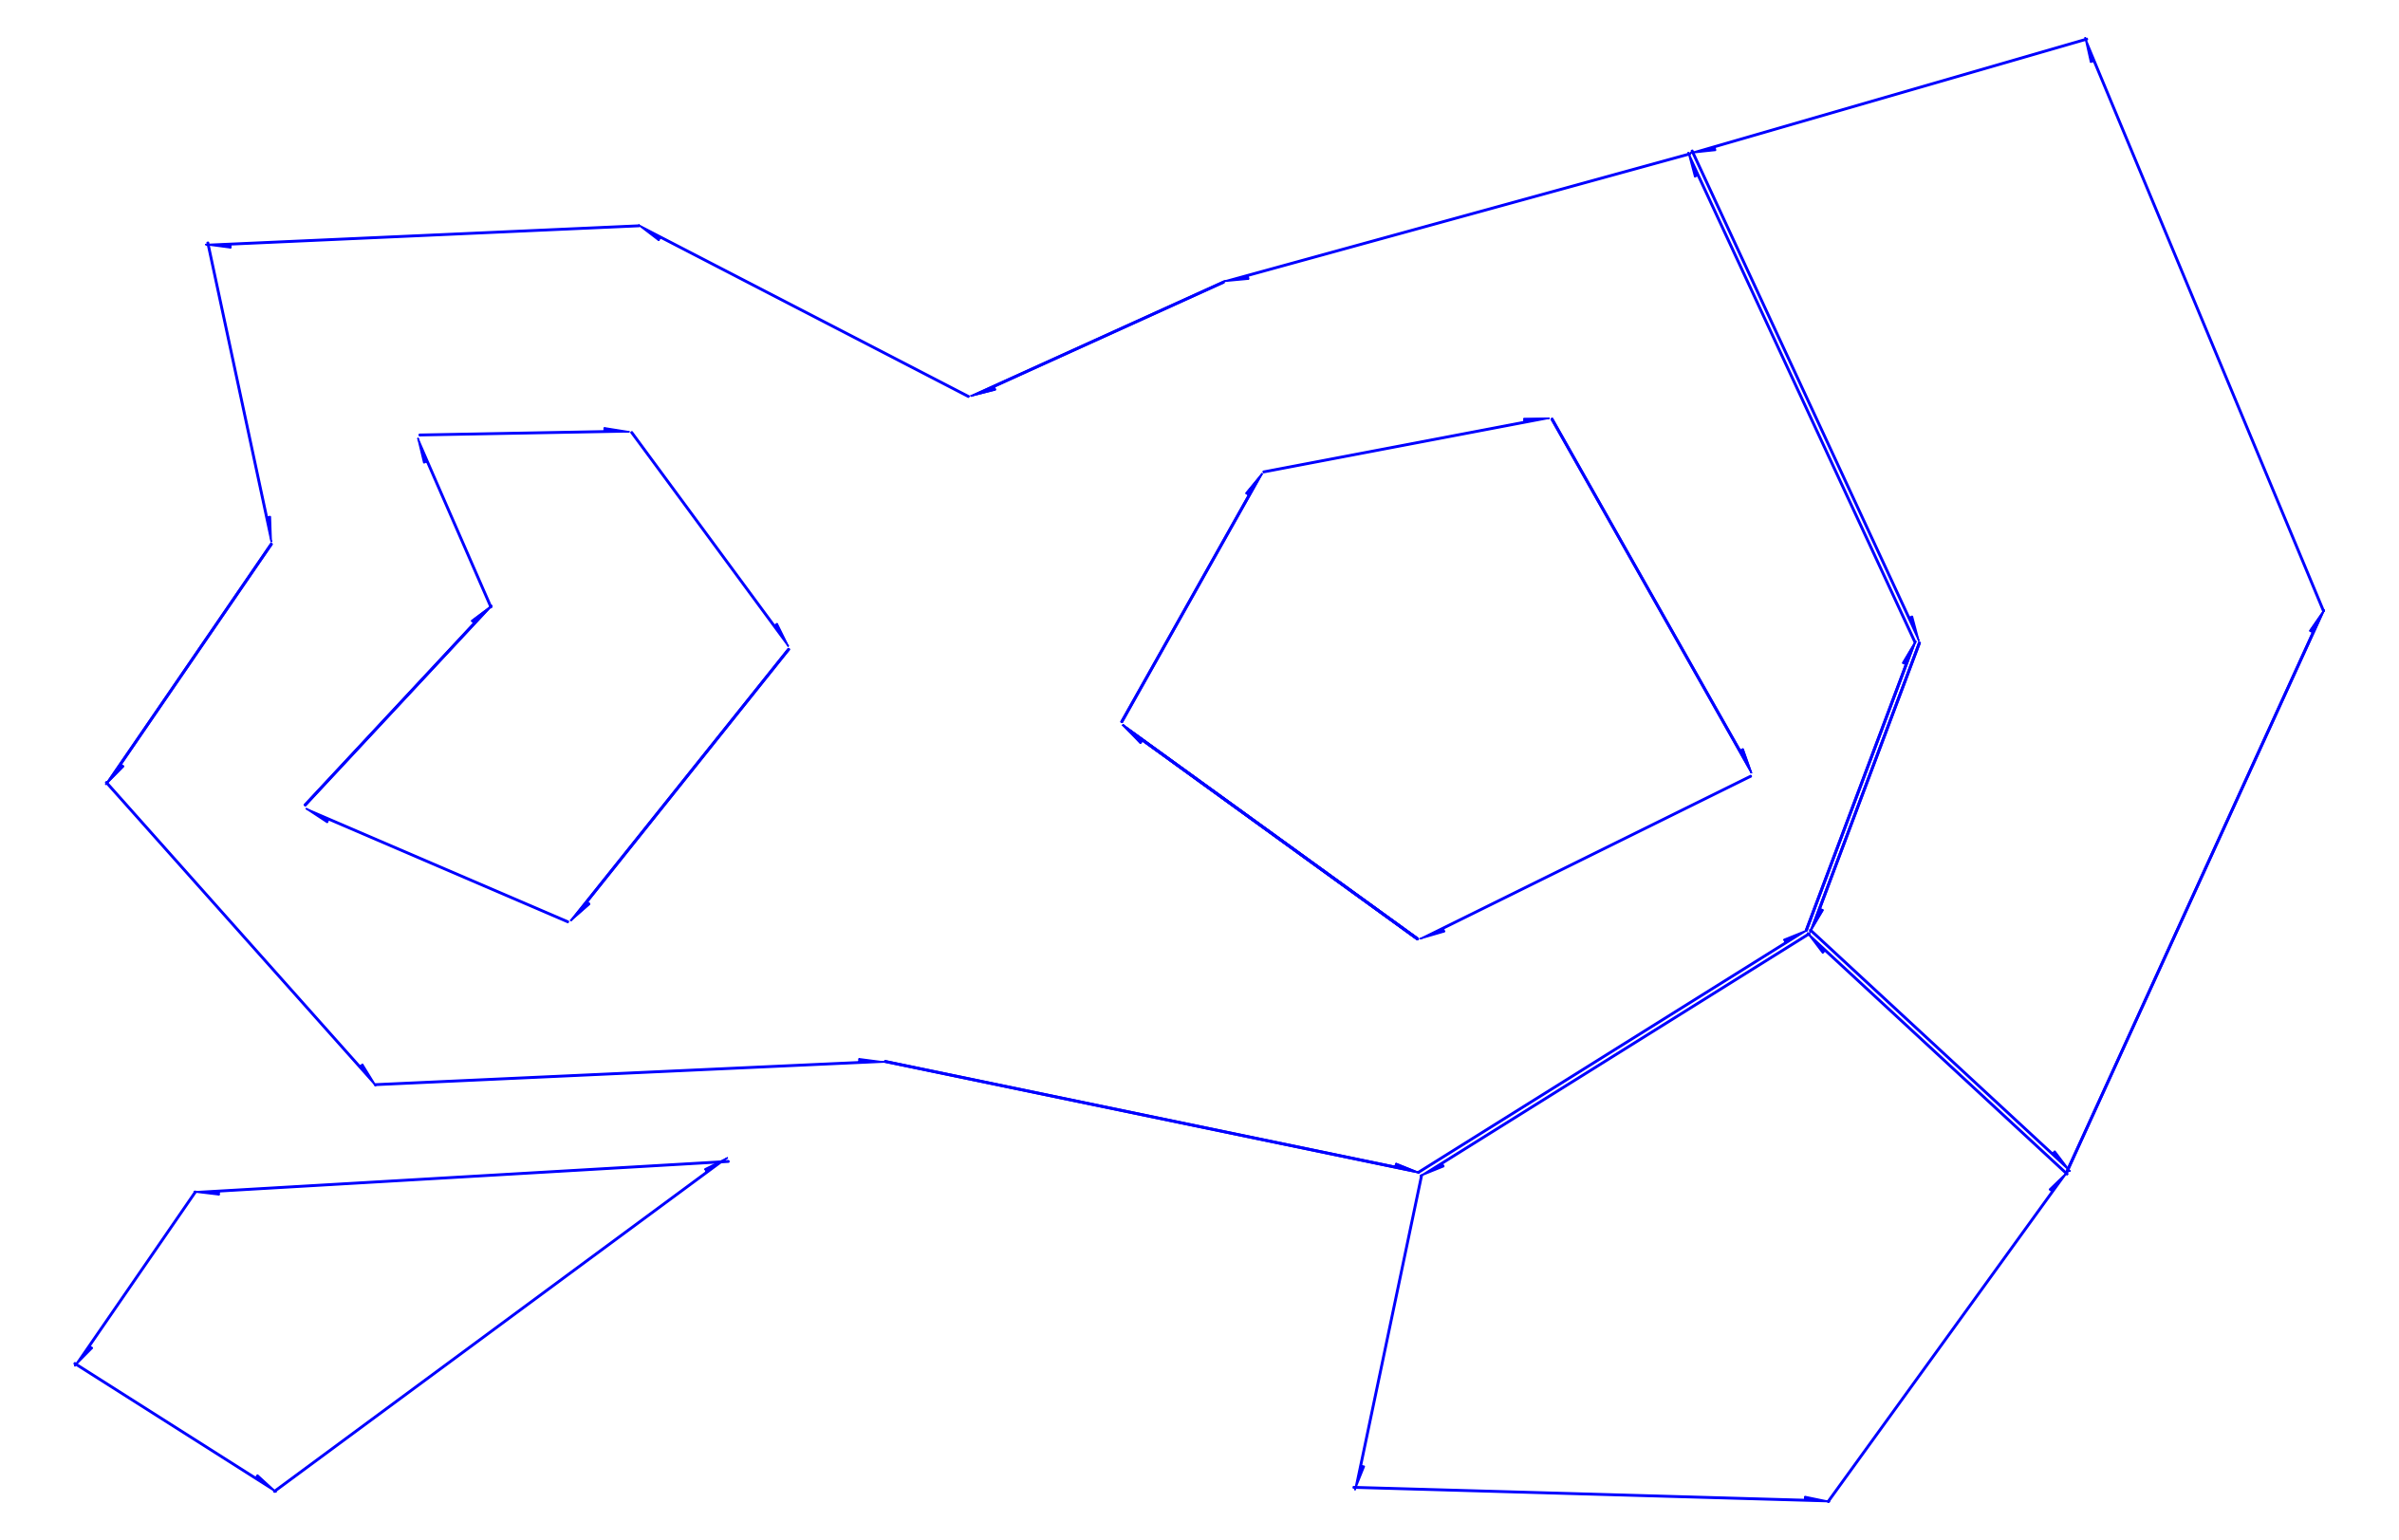
\includegraphics[width=0.8\linewidth]{figures/EP02}     
\end{frame}

\begin{frame}{Partitions}
    \centering 
    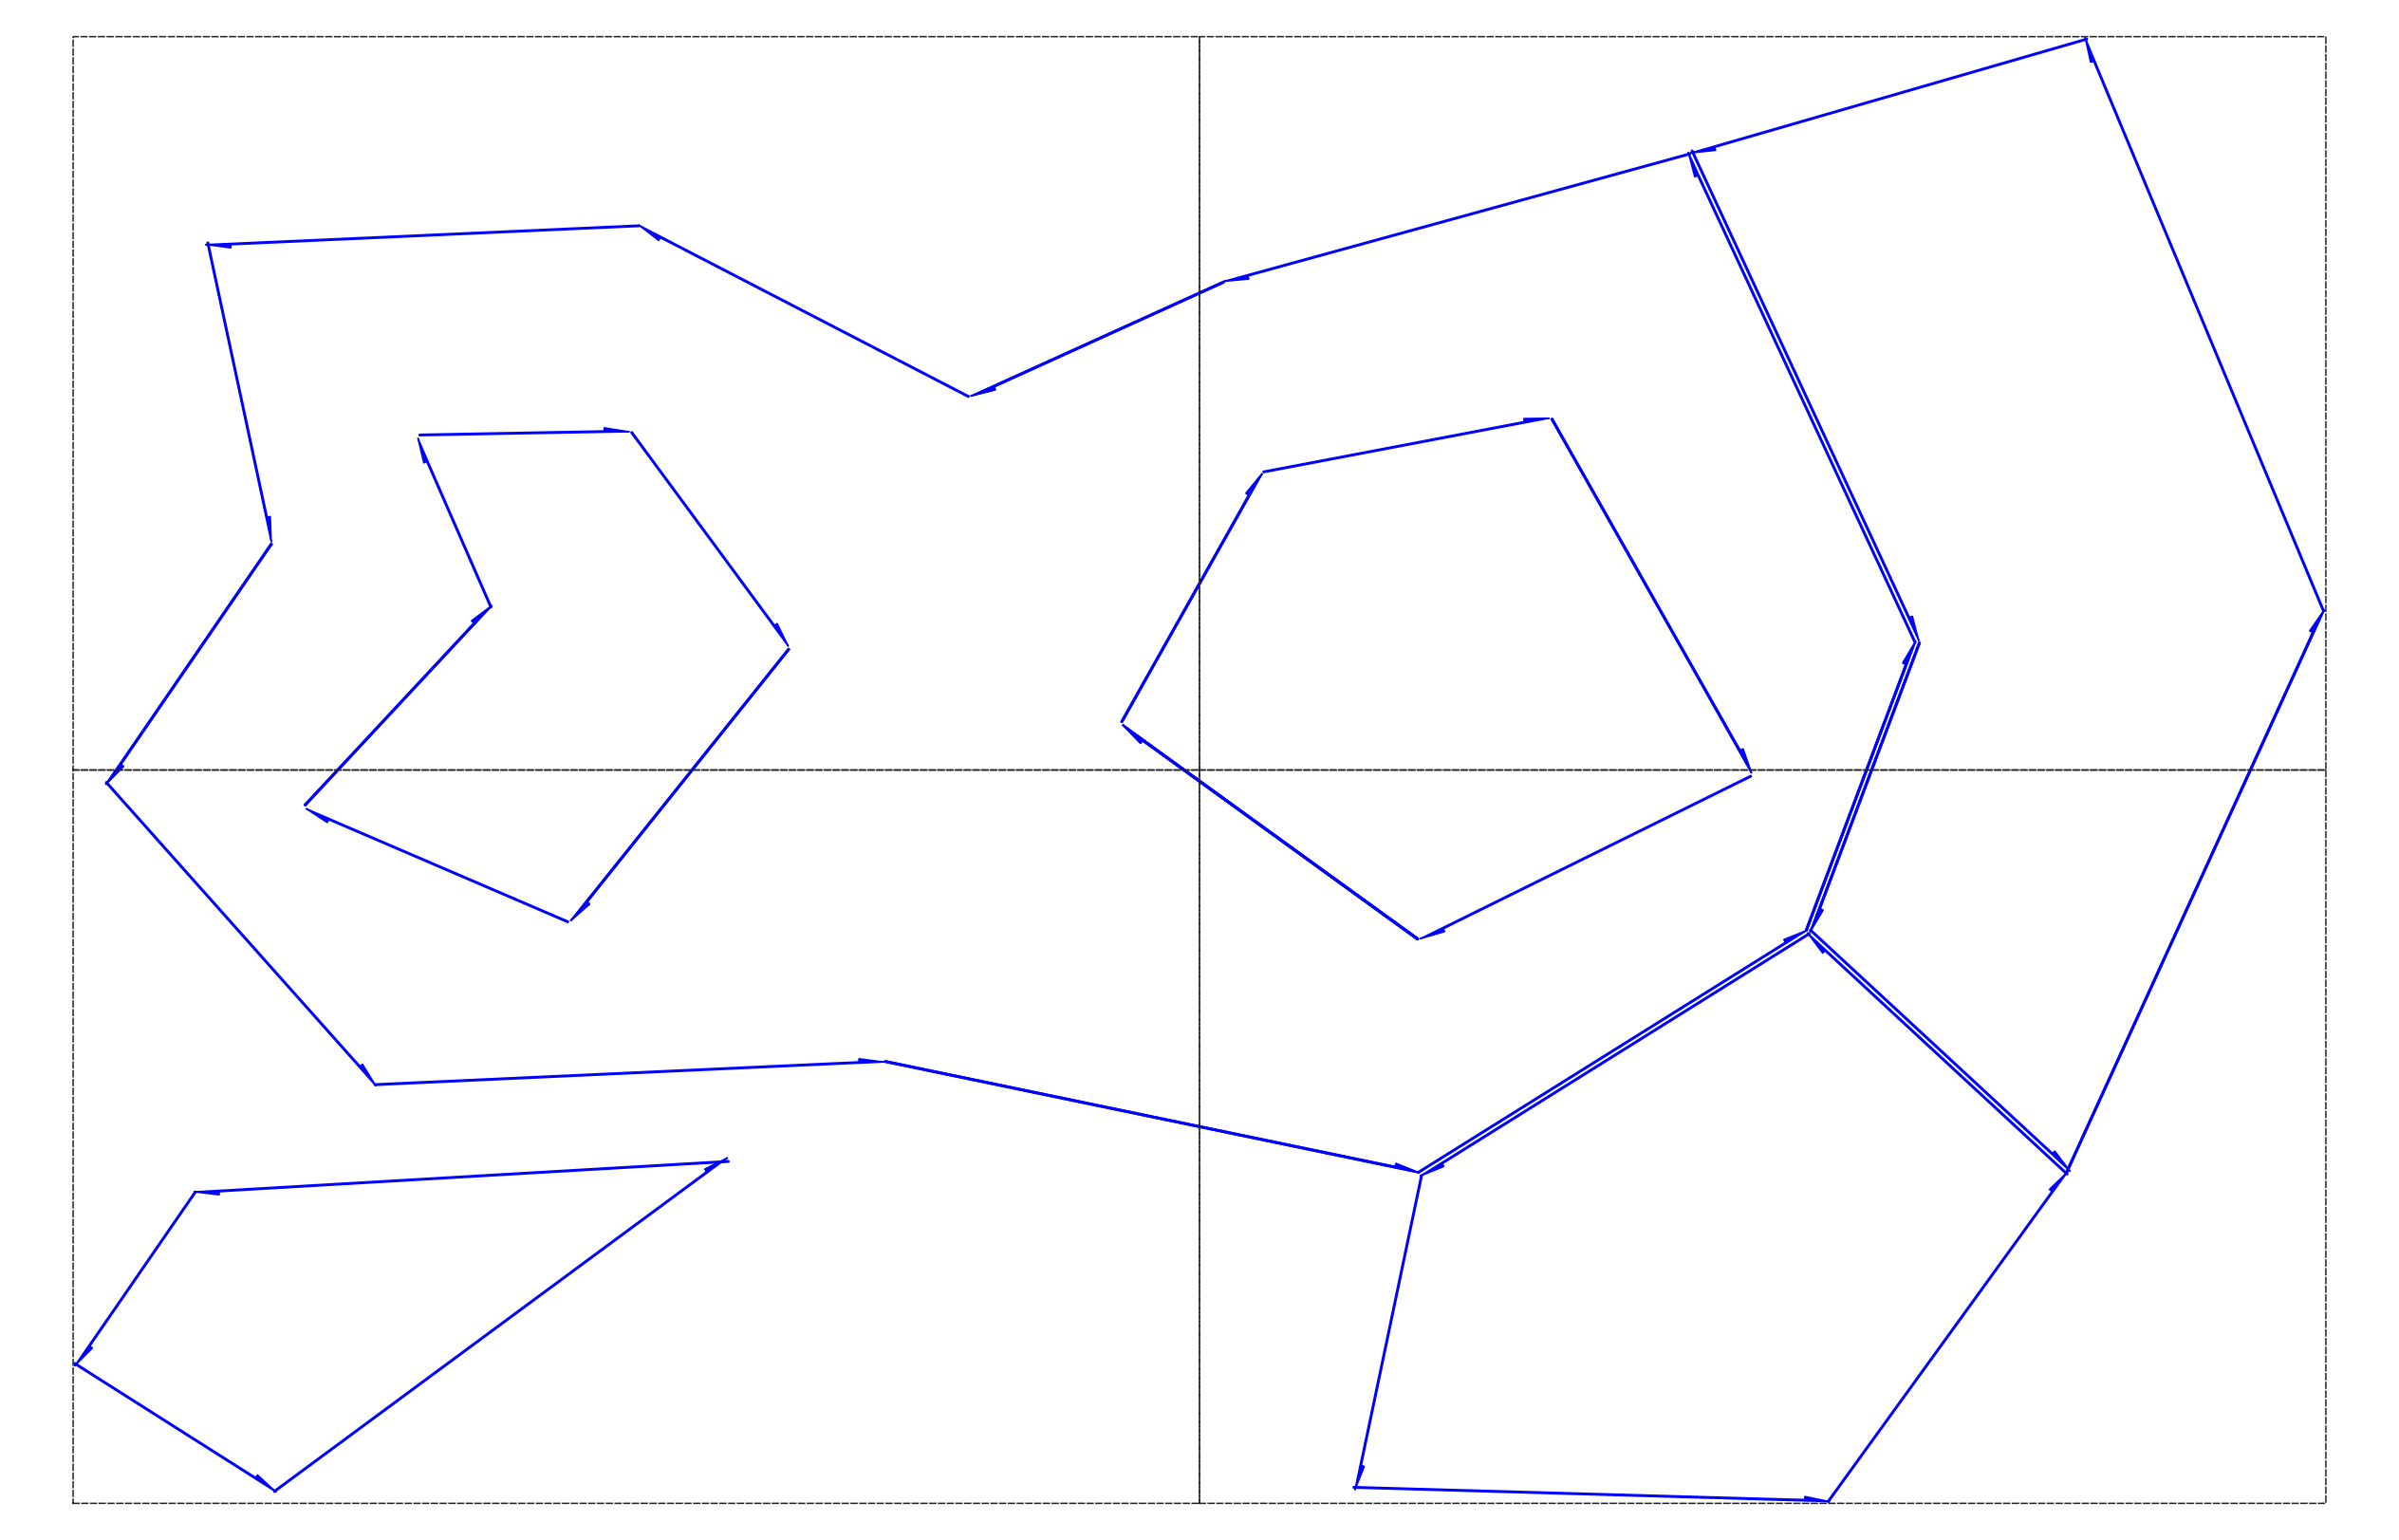
\includegraphics[width=0.8\linewidth]{figures/EP03}     
\end{frame}

\begin{frame}{Extract cell edges}
    \centering 
    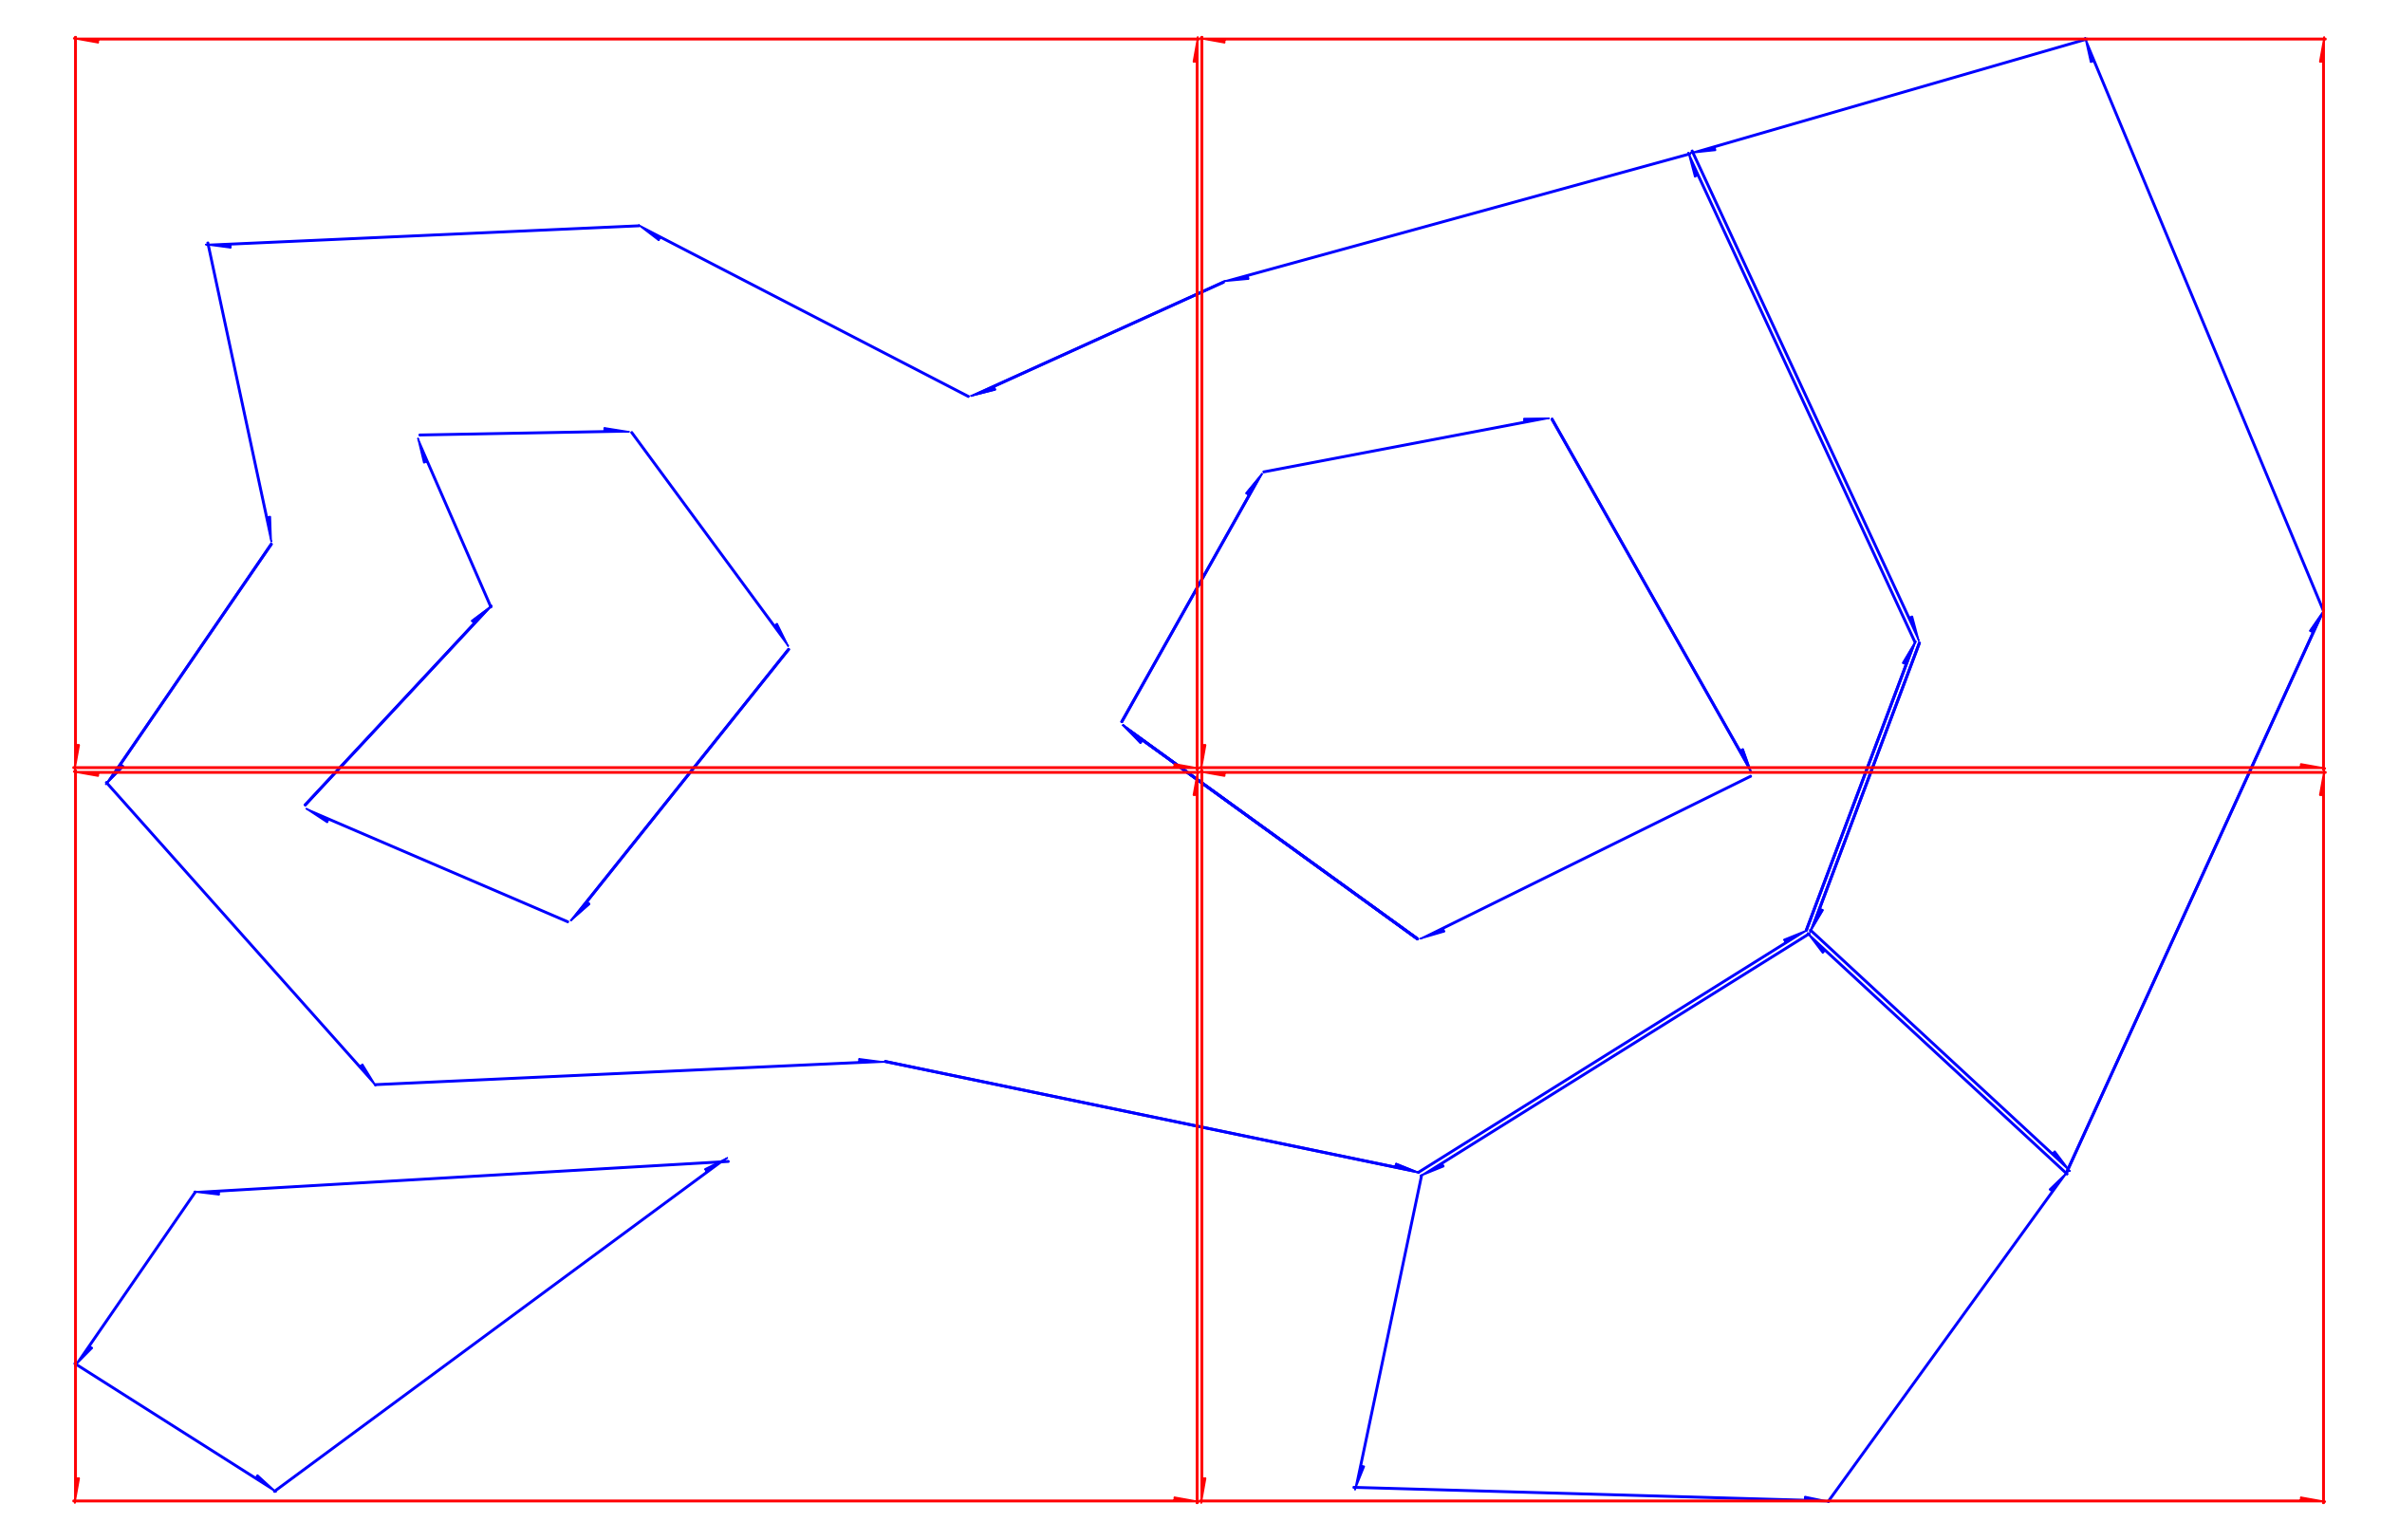
\includegraphics[width=0.8\linewidth]{figures/EP04}     
\end{frame}

\begin{frame}{Merge and find intersections}
    \centering 
    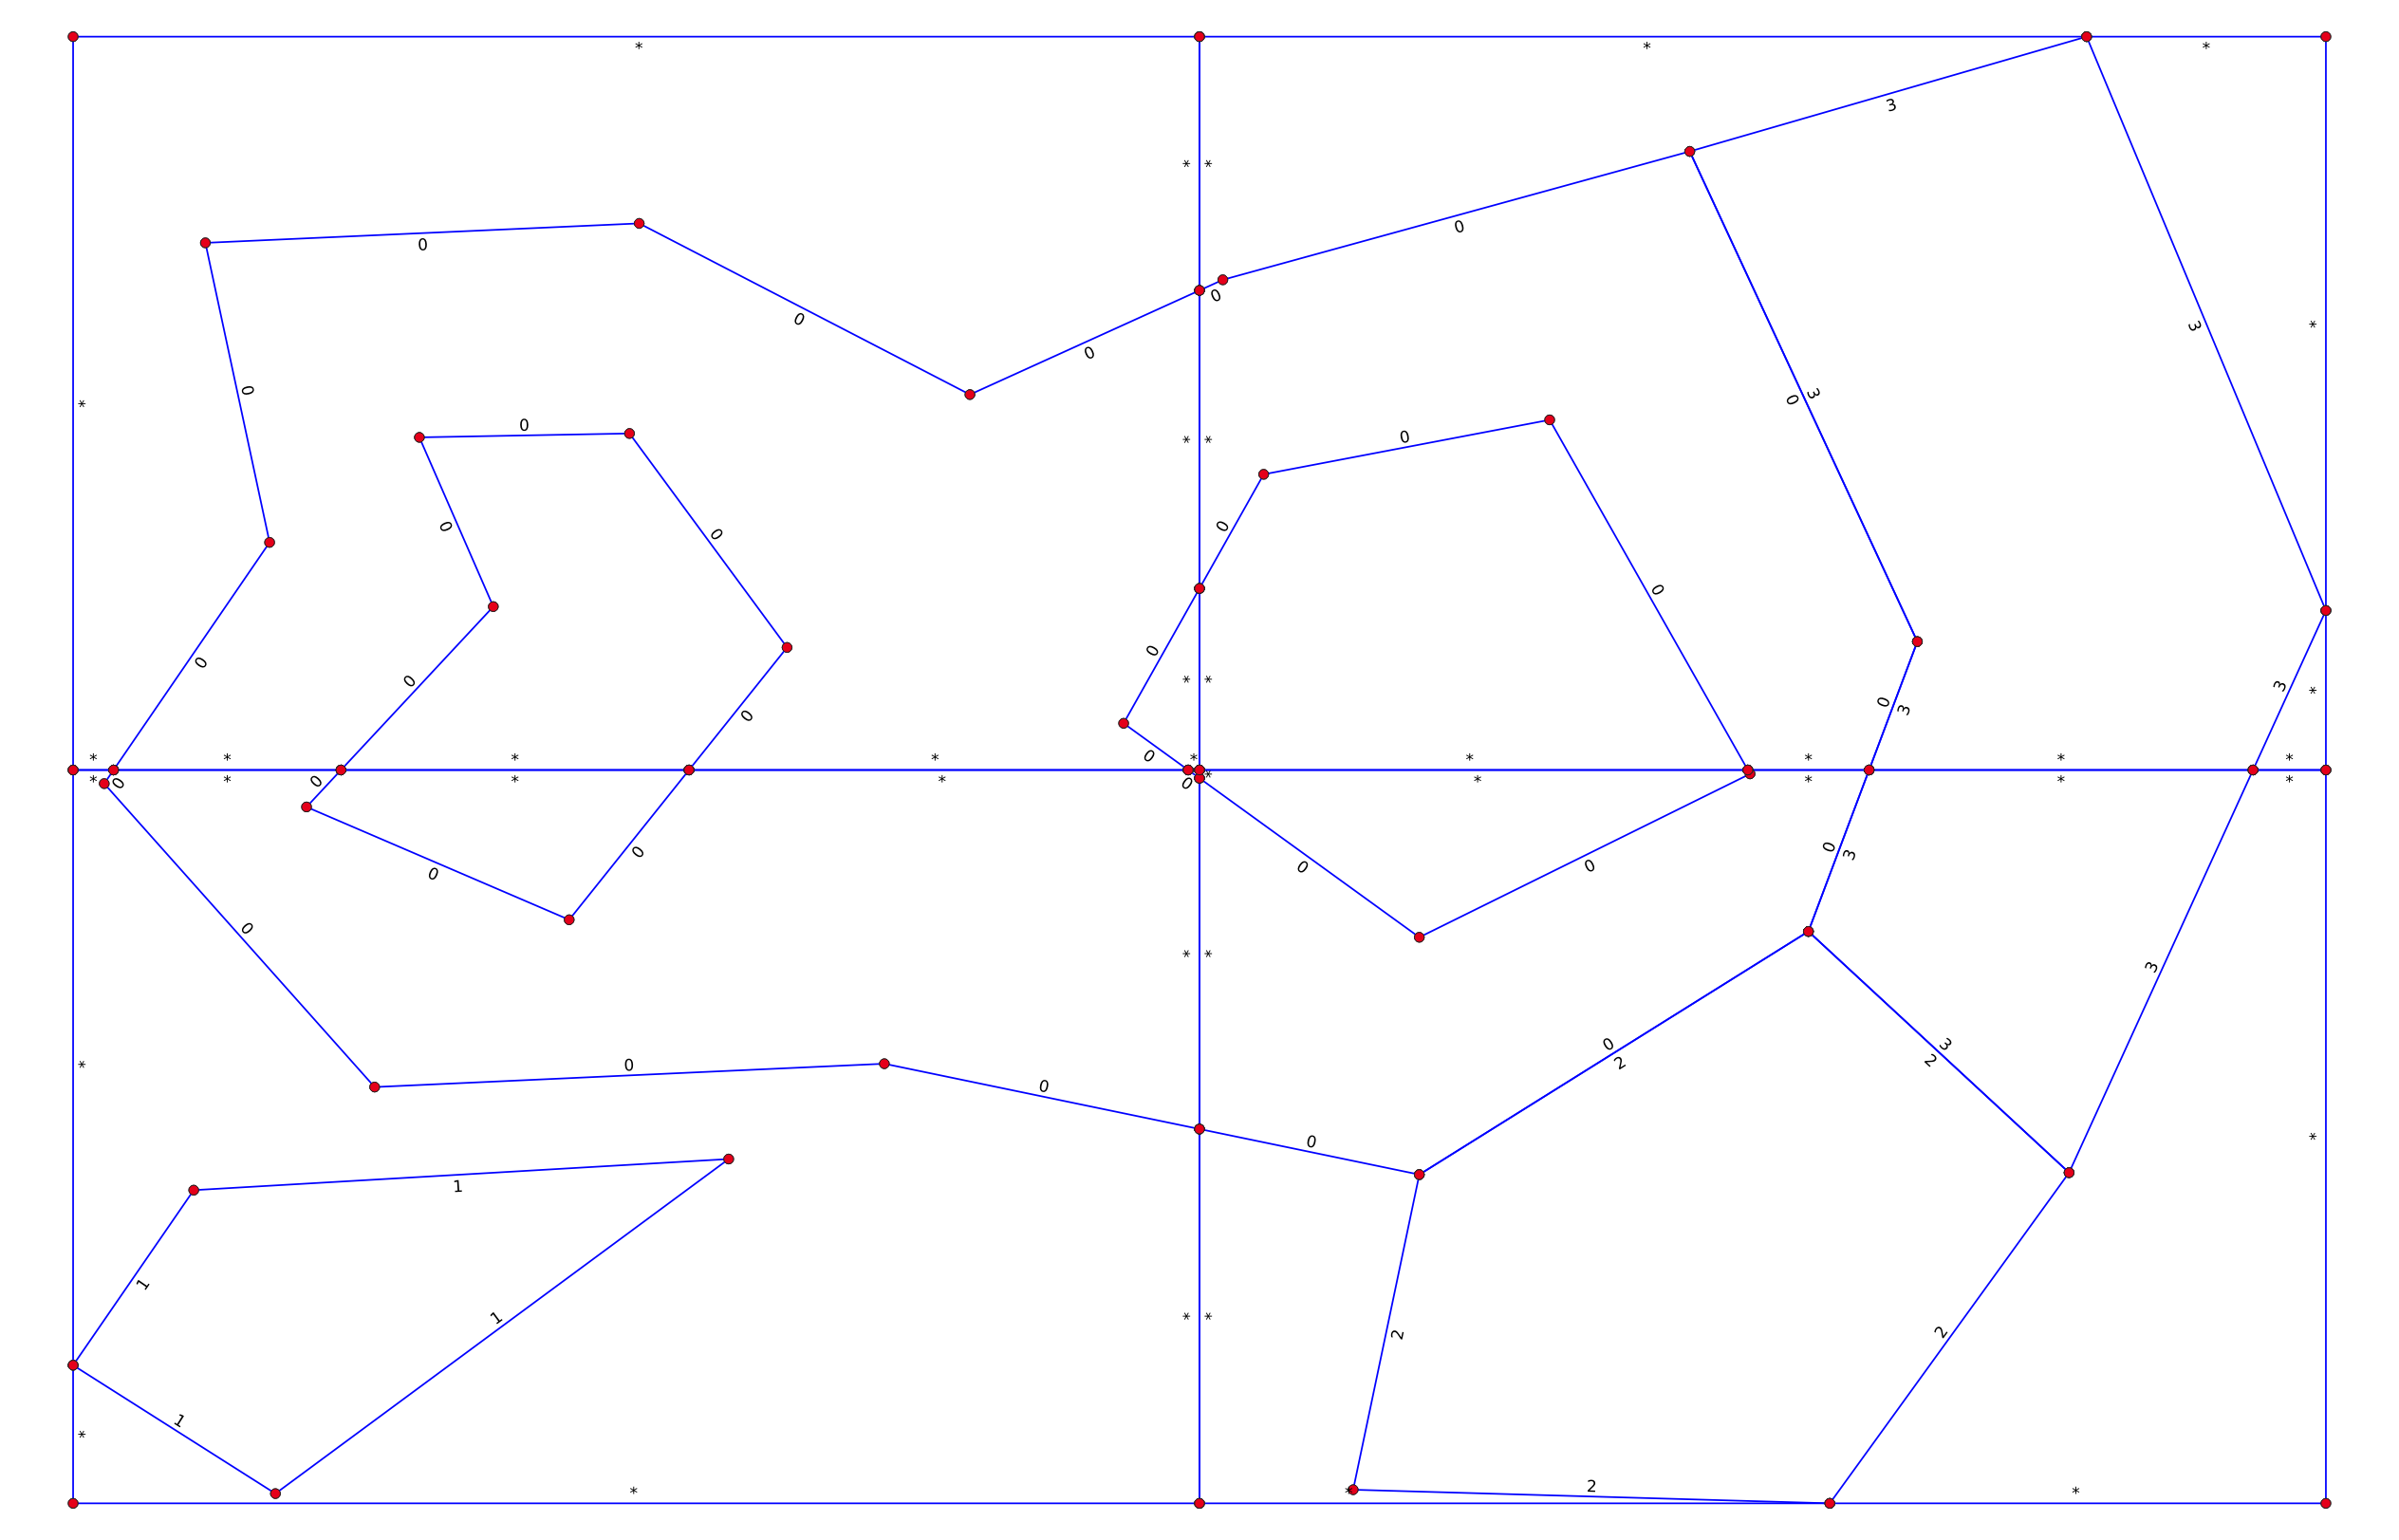
\includegraphics[width=0.8\linewidth]{figures/EP05}     
\end{frame}

\begin{frame}{Build local DCEL's}
    \centering 
    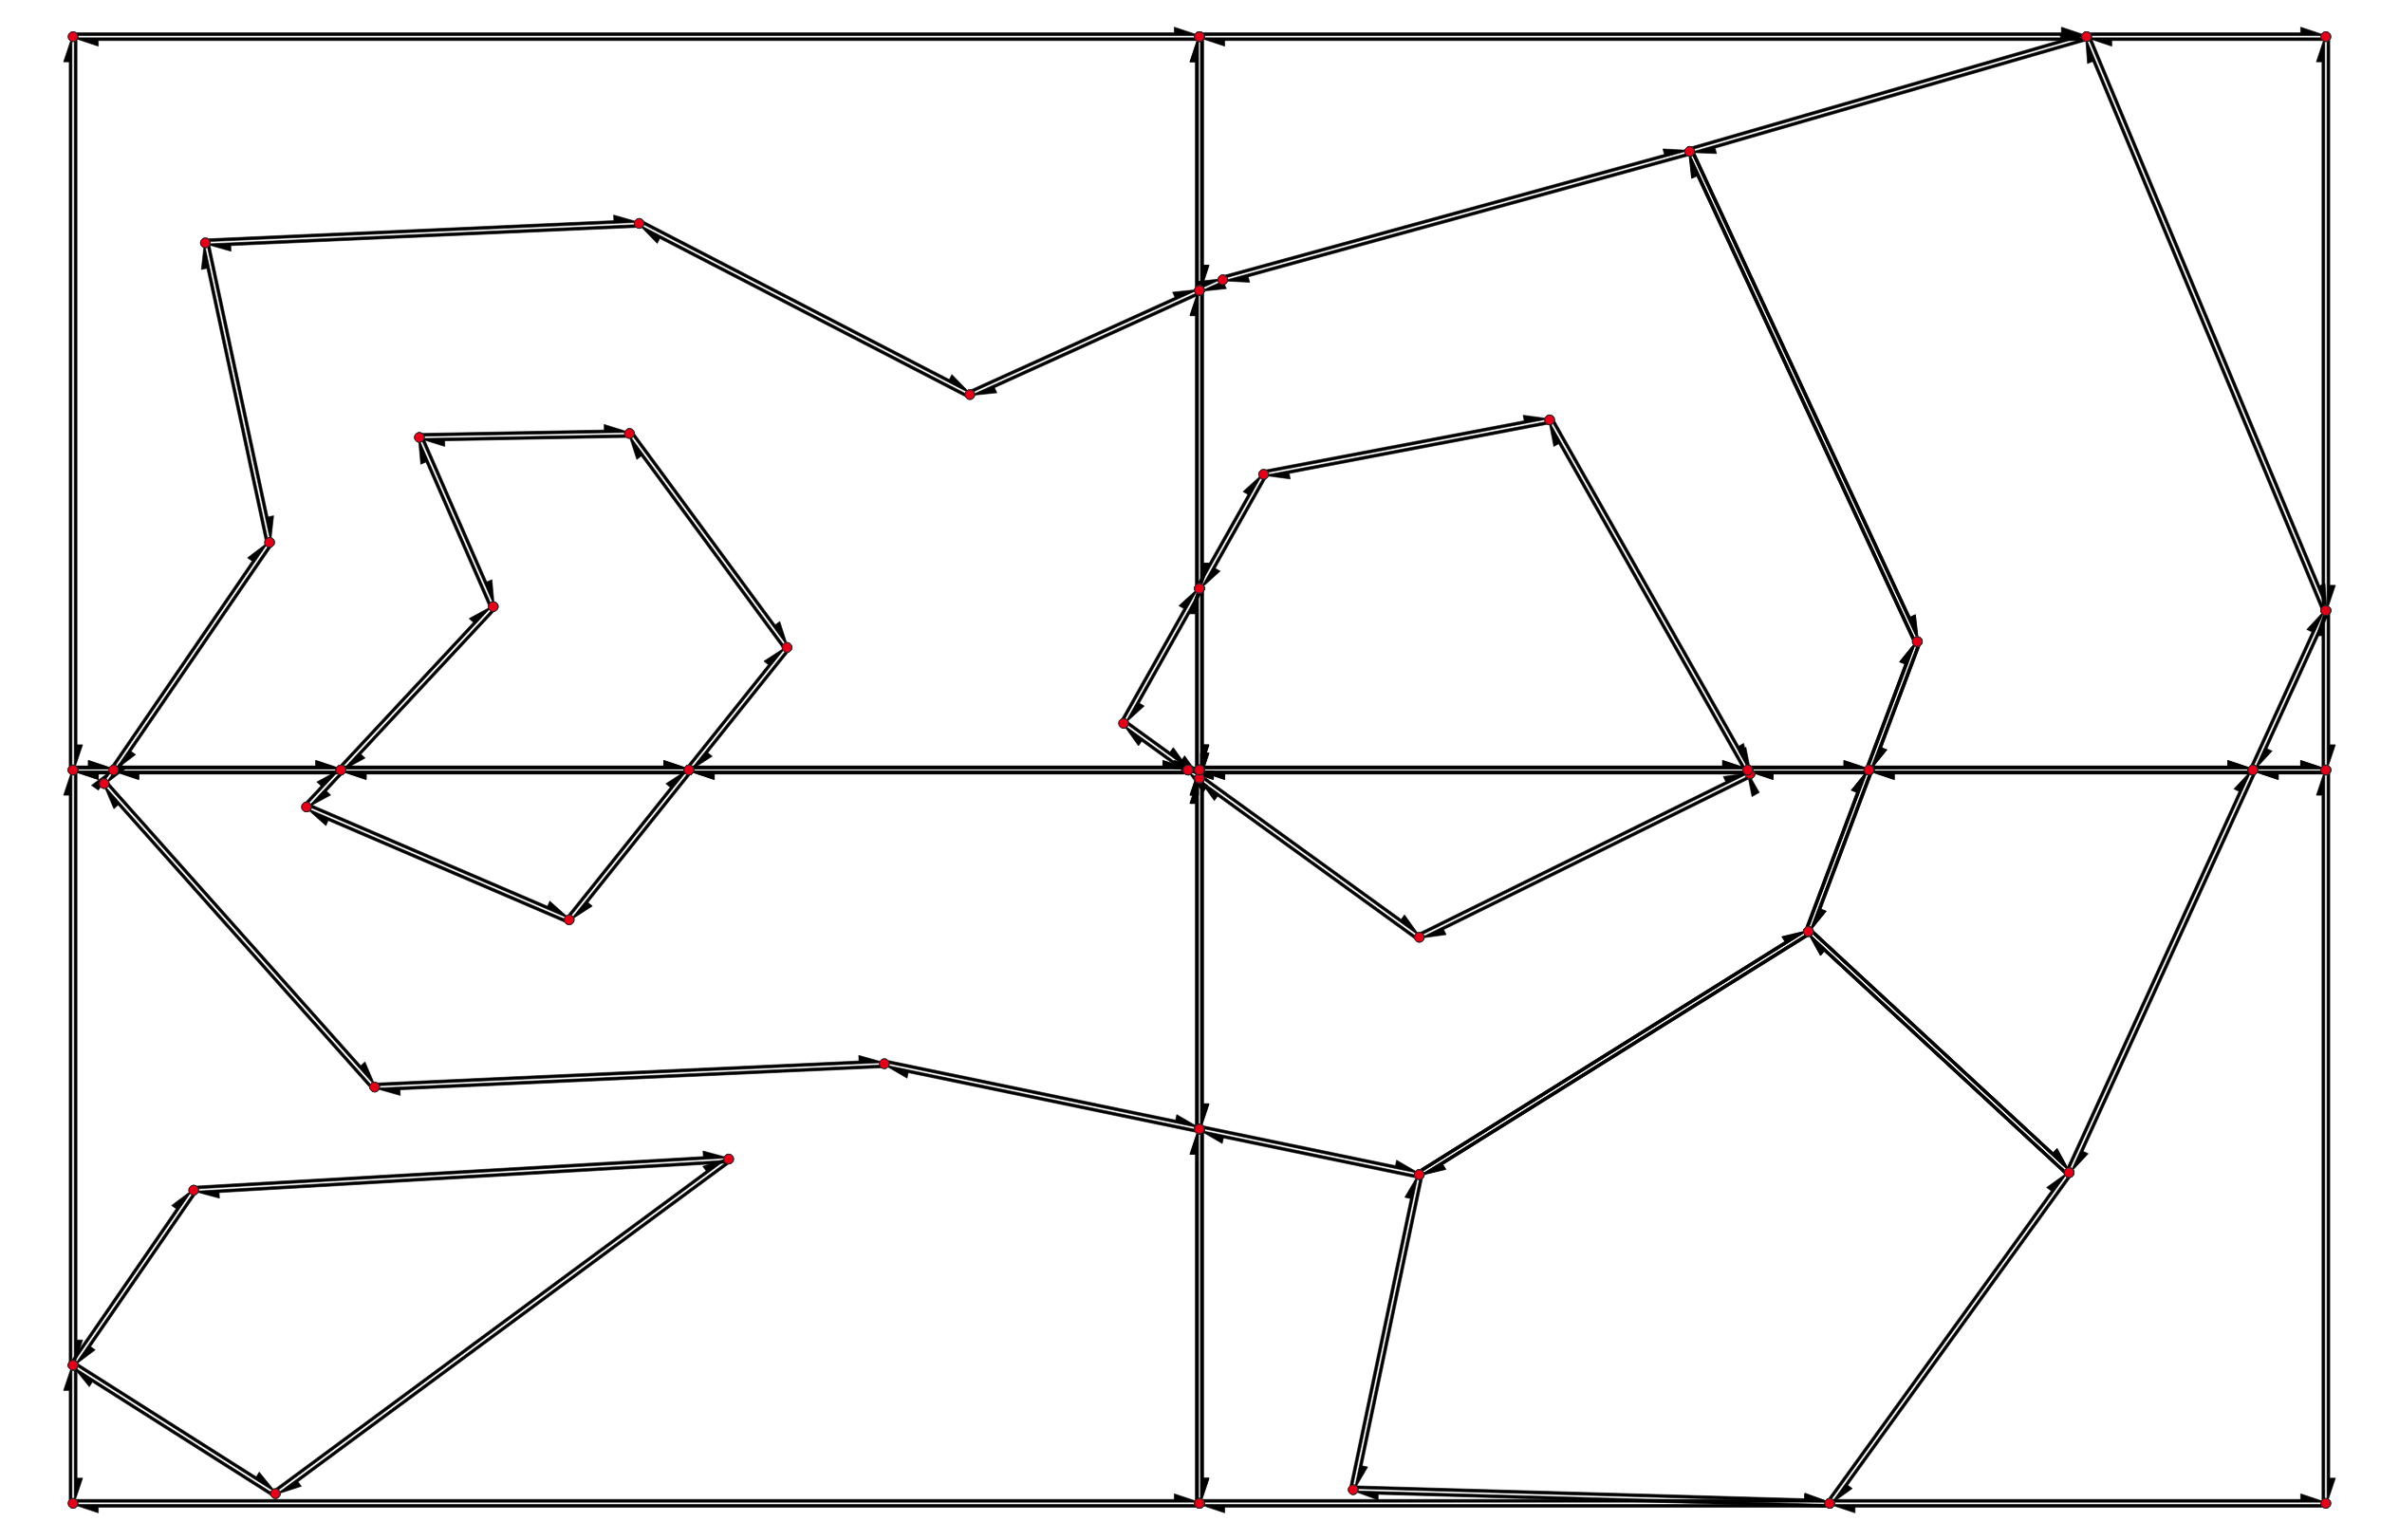
\includegraphics[width=0.8\linewidth]{figures/EP06}     
\end{frame}

\begin{frame}{What is next?}
    \begin{itemize}
        \item Finish local DCEL contruction.
        \item Test improvement versus previous implementation.
        \item Integrate the code.
    \end{itemize}
\end{frame}

\end{document}
